% Options for packages loaded elsewhere
\PassOptionsToPackage{unicode}{hyperref}
\PassOptionsToPackage{hyphens}{url}
%
\documentclass[
]{article}
\usepackage{lmodern}
\usepackage{amssymb,amsmath}
\usepackage{ifxetex,ifluatex}
\ifnum 0\ifxetex 1\fi\ifluatex 1\fi=0 % if pdftex
  \usepackage[T1]{fontenc}
  \usepackage[utf8]{inputenc}
  \usepackage{textcomp} % provide euro and other symbols
\else % if luatex or xetex
  \usepackage{unicode-math}
  \defaultfontfeatures{Scale=MatchLowercase}
  \defaultfontfeatures[\rmfamily]{Ligatures=TeX,Scale=1}
\fi
% Use upquote if available, for straight quotes in verbatim environments
\IfFileExists{upquote.sty}{\usepackage{upquote}}{}
\IfFileExists{microtype.sty}{% use microtype if available
  \usepackage[]{microtype}
  \UseMicrotypeSet[protrusion]{basicmath} % disable protrusion for tt fonts
}{}
\makeatletter
\@ifundefined{KOMAClassName}{% if non-KOMA class
  \IfFileExists{parskip.sty}{%
    \usepackage{parskip}
  }{% else
    \setlength{\parindent}{0pt}
    \setlength{\parskip}{6pt plus 2pt minus 1pt}}
}{% if KOMA class
  \KOMAoptions{parskip=half}}
\makeatother
\usepackage{xcolor}
\IfFileExists{xurl.sty}{\usepackage{xurl}}{} % add URL line breaks if available
\IfFileExists{bookmark.sty}{\usepackage{bookmark}}{\usepackage{hyperref}}
\hypersetup{
  pdftitle={Honors Draft},
  pdfauthor={Raven McKnight},
  hidelinks,
  pdfcreator={LaTeX via pandoc}}
\urlstyle{same} % disable monospaced font for URLs
\usepackage[margin=1in]{geometry}
\usepackage{graphicx,grffile}
\makeatletter
\def\maxwidth{\ifdim\Gin@nat@width>\linewidth\linewidth\else\Gin@nat@width\fi}
\def\maxheight{\ifdim\Gin@nat@height>\textheight\textheight\else\Gin@nat@height\fi}
\makeatother
% Scale images if necessary, so that they will not overflow the page
% margins by default, and it is still possible to overwrite the defaults
% using explicit options in \includegraphics[width, height, ...]{}
\setkeys{Gin}{width=\maxwidth,height=\maxheight,keepaspectratio}
% Set default figure placement to htbp
\makeatletter
\def\fps@figure{htbp}
\makeatother
\setlength{\emergencystretch}{3em} % prevent overfull lines
\providecommand{\tightlist}{%
  \setlength{\itemsep}{0pt}\setlength{\parskip}{0pt}}
\setcounter{secnumdepth}{5}
\usepackage{float}
\usepackage{booktabs}

\title{Honors Draft}
\author{Raven McKnight}
\date{2/9/2020}

\begin{document}
\maketitle
\begin{abstract}
abstract
\end{abstract}

\hypertarget{introduction}{%
\section{Introduction}\label{introduction}}

Public transit ridership has been in decline around the country for
years, but particularly since the mid 2010s (). Following a spike in
ridership related to the 2008 housing market crash, ridership has been
steadily trending downwards in most metropolitan areas (). Bus ridership
is particularly affected compared to more ``desirable'' light rail and
commuter rail. Transit agencies are naturally interested in
understanding the specific causes of these declines, as well as more
generally being able to predict transit demand throughout space and
time.

Transit ridership, or demand, is often forecasted using models from the
policy and planning world, such as the classic four-step model.
Four-step transportation demand models consist of simulating trips and
their spatial distribution before assigning them modes (ie bus versus
car versus bicycle) and routes. Other models, called activity-based
models predict transportation demand based on when and where riders are
likely to conduct various tasks (commuting, shopping, recreation, etc).
Others still are based largely on land-use characteristics under the
general premise that different types of development (or lack thereof)
are more or less likely to draw riders.

It is somewhat rare to see more traditional statistical models applied
to transit ridership. In the context of predicting future ridership, the
above methods are often sufficient. Additionally, they are the industry
standard and allow for the integration of expert planning knowledge.
However, in the context of understanding \emph{past} ridership, we can
apply more explanatory methods. Specifically, we can use hierarchical
spatial Bayesian models to incorporate many covariates in addition to
the spatial structure that necessarily underpins transit ridership (ie,
boardings can only occur at existing bus stops).

Hierarchical spatial models allow us to understand the patterns of
ridership within a city with great granularity. Some existing literature
explores the decline of transit ridership \emph{between} cities (). Few
studies have been conducted on the various patterns of ridership
\emph{within} a single metropolitan area. Additionally, few studies
incorporate many demographic predictors. Naturally, we cannot collect
demographic information for every rider of a transit system. Instead, we
can use demographic predictors associated with spatial units such as
census block groups to explore the question of \emph{who} rides -- or,
at the very least, \emph{where} do they ride.

\hypertarget{background}{%
\section{Background}\label{background}}

\hypertarget{metro-transit}{%
\subsection{Metro Transit}\label{metro-transit}}

Metro Transit is the primary transit provider in the Minneapolis-Saint
Paul metropolitan area. The agency operates one commuter rail line
(Northstar), two light rail lines (Blue Line and Green Line), and over
100 bus routes. Since the 2014 opening of the Green Line, rail ridership
has increased each year (). Bus ridership, however, has been in decline.
According to the Metro Transit Riders' Almanac blog, much of the decline
is bus ridership can be attributed to the busiest urban local routes as
well as situational factors, such as lower-than-average gas prices and a
system-wide fare increase in 2017.

The agency is naturally interested in understanding with more detail the
reasons for and nature of these declines.

Conducted in tandem with Metro Transit's Network Next bus system
redesign, this study aims to further Metro Transit's understanding of
their bus network. Specifically, we aim to describe the existing pattern
of transit ridership via demographic predictors and spatial patterns.
Future work will incorporate temporal trends to better understand
declining ridership.

\hypertarget{transit-market-areas}{%
\subsection{Transit Market Areas}\label{transit-market-areas}}

Metro is interested in predicting transit demand across the region in
order to guide route planning and service provision. Currently, Metro
Transit uses a set of 5 Transit Market Areas to estimate spatial demand.
The Transit Market Areas are writen into the official Transportation
Planning Policy (TPP) and are calculated using a simple linear
regression. Following the notation of the TPP, the formula for determing
Transit Market Areas is expressed

\[
\begin{aligned}
\text{Transit Market Index } = & \text{ 0.64 * Population Density + 0.20 * Employment Density +} \\
& \text{0.23 * Intersection Density + 0.11 * Automobile Availability}
\end{aligned}
\]

where each predictor is logged and scaled by developed land acreage per
census block group. Here, automobile availability refers to the number
of adults over age 16 less the total number of automobiles available in
a block group (scaled by developed land acreage). There is an additional
indicator variable, omitted in this notation, for the census block group
containing the MSP International Airport. For more documentation of the
official Transit Market Areas, refer to the TPPs
\href{https://metrocouncil.org/Transportation/Planning-2/Key-Transportation-Planning-Documents/Transportation-Policy-Plan/The-Adopted-2040-TPP-(1)/Final-2040-Transportation-Policy-Plan/2040-TPP-Appendix-G-Transit-Design-and-Perf-Standa.aspx}{Appendix
G}.

\begin{figure}[htb]
  \centering
  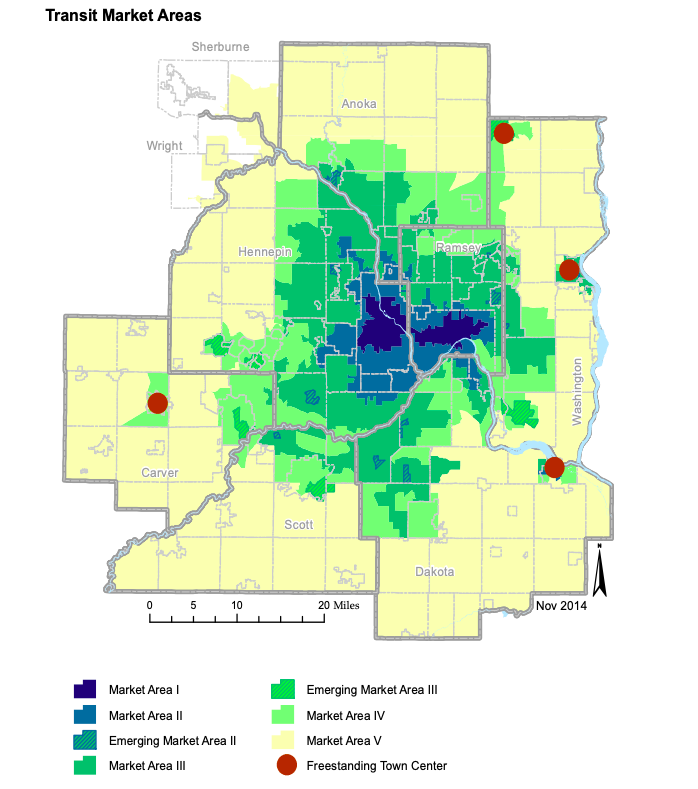
\includegraphics[width = 5in]{TMA.png}
  \caption{Metro Transit's Transit Market Areas from Metropolitan Council's Transportation Planning Policy, Appendix G. }
\end{figure}

Census block groups are split into 5 market areas based on the Transit
Market Index described above, where the highest market area (Market Area
1) is expected to support high-frequency, all-day service and the lowest
market area (Market Area 5) is expected to support peak commuter express
service and park-and-rides, if that.

The Transit Market Index values are geographically smoothed to create
more-or-less concentric Transit Market Areas. The linear regression is
an intuitive way to think about transit ridership across space. The four
predictors used are common-sense indicators of transit ridership: high
population and employment density are characteristic of trip origins and
destinations, automobile availability is reasonably assumed to be
related to transit ridership, and intersection density is a proxy for
the ``walkability'' of an area. However, the exsiting Transit Market
Area model may be over-simplifying the complex question of transit
ridership.

\hypertarget{data}{%
\section{Data}\label{data}}

\hypertarget{metro-transit-data}{%
\subsection{Metro Transit Data}\label{metro-transit-data}}

This analysis relies on several Metro Transit provided data sets. The
two primary sources are automatically reported by in-service vehicles,
yielding billions of rows of observations.

\textbf{Automatic Passenger Count (APC)} data is reported every time a
bus opens its doors. Two beams of light detect movement through the
doors of the bus and counts the number of passengers getting on and off
at each bus stop. Naturally, this data source is flawed: sometimes,
vehicles fail to report data, and the sensors can be easily tricked.
Someone getting off the bus pulling a suitcase behind them, for example,
would likely be counted as two passengers exiting. However, APC is the
most granular ridership data available, giving us the most control over
our spatial aggregations of ridership. This is the primary data source
used in this analysis.

\textbf{Automatic Vehicle Location (AVL)} data is similarly reported by
in-service vehicles (approximately) every 8 seconds. The vehicle reports
in GPS location continuously while in service. We use AVL data to adjust
for missing APC data.

\textbf{Metro Transit's Schedule} as \emph{planned}, rather than as
\emph{run}, is also used to correct missing APC data.

This analysis began by pulling all APC, AVL, and schedule data from
2015-2018. The initial data pull consisted of approximately 496
\emph{billion} rows of data. The analysis presented here focuses on 2017
data. Figure *\_\_\_* shows the average weekday boardings by census
block group in 2017.

\begin{figure}[H]
  \centering
  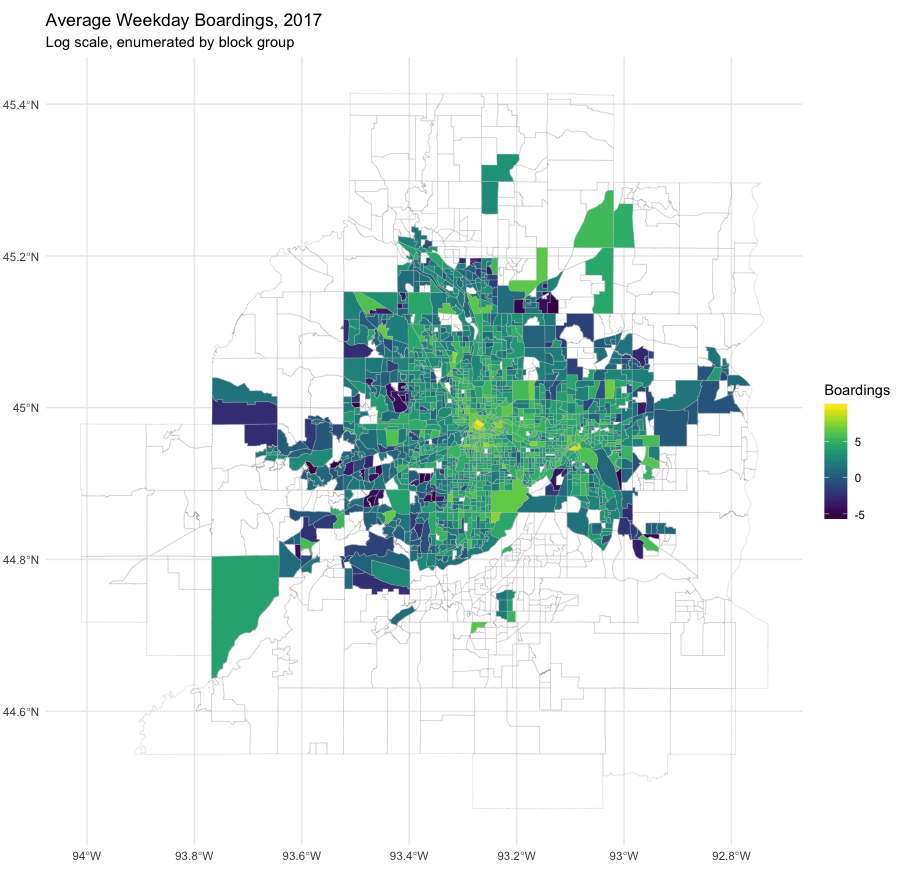
\includegraphics[width = 5in]{weekdayboardings.png}
  \caption{Average weekday boardings by census block group, the response variable for this analysis.}
\end{figure}

\hypertarget{data-interpolation}{%
\subsubsection{Data Interpolation}\label{data-interpolation}}

In theory, we have APC data for each run bus trip in 2017. However, we
know that, for a variety of reasons, this is untrue. The automatic data
reporting technology on Metro Transit buses is flawed and can fail to
report data unpredictably. Additionally, the trips missing data may not
be random: all buses of one ``series'', for example, may fail to report
at once. This could lead to the APC dataset understimating boardings on
a particular set of routes or locations.T herefore, we use the three
data sets described above to create a more complete augmented APC data
set.

The algorithm used to interpolate data works essentially as follows:

\begin{enumerate}
\def\labelenumi{\arabic{enumi}.}
\tightlist
\item
  Compares scheduled trips to trips we have APC data for. If a trip was
  scheduled but has no APC records, we consider that trip missing.
\item
  For missing trips, check AVL data. If there are no AVL records, we
  consider the trip cut (ie, we assume the trip was not run).
\item
  For missing trips with AVL data, we estimate boardings for that trip
  by taking the average number of boardings for trips of that nature
  (trips on the same route, day of week, season, location, etc).
\end{enumerate}

\hypertarget{data-aggregation}{%
\subsubsection{Data Aggregation}\label{data-aggregation}}

For the models presented in this study, we aggregate boardings at
individual bus stops to the census block group. This is in large part to
match the granularity of the American Community Survey covariates we are
interested in using. Future work could explore using areal covariates to
model ridership at specific points (ie, bus stops).

Additionally, we aggregate boardings counts to average weekday
boardings. This a) greatly reduces the number of rows of data in play,
and therefore shortens computation time significantly, and b) allows us
to build a spatial model without simultaneously incorporating temporal
trends. The data interpolation described above will be more impactful in
future studies incorporating temporal trends.

\hypertarget{other-data-sources}{%
\subsection{Other data sources}\label{other-data-sources}}

All other data sources used in this study are from outside sources.
Census Block Groups are used as the areal unit of analysis. Covariates
of interest are primarily from the 2017 American Community Survey (ACS)
5-Year Estimates. Additional variables related to employment are sourced
from the Longitudinal Origin-Destination Employment Statistics (LODES)
dataset. A full list of covariates used in this study is below.

\begin{table}[H]
\centering
\begin{tabular}{ll} \toprule
    Parameter & Meaning \\ \midrule
    beta[1] & median household income \\ 
    beta[2] & percent residents identified as white alone \\ 
    beta[3] &  area of 10 minute walk isochrone from population-weighted block group centroid \\
    beta[4] &  percent residents with a high school diploma \\
    beta[5] &  percent residents with a bachelor's degree \\
    beta[6] &  percent of residents who rent their residence \\
    beta[7] &  percent of residents without a vehicle \\
    beta[8] &  percent of residents who speak only English \\
    beta[9] &  percent of residents identified as foreign \\
    beta[10] & employment density \\
    beta[11] & percent of jobs in block group for white employees \\
    beta[12] & percent of jobs in block group for male employees \\
    beta[13] & percent of jobs in block group for employees with no college degree \\
    beta[14] & percent of jobs in block group for employees who make less than \$40,000 \\
    beta[15] & percent of jobs in block group for employees under age 30 \\
    beta[16] & median age \\
    beta[17] & percent residents who use transit to commute to work \\
    beta[18] & population density \\
    \bottomrule
 \hline
\end{tabular}
\caption{List of covariates}
\end{table}

Note that \texttt{beta{[}3{]}} is a measure of walkability. A 10-minute
walk isochrone, generated using OpenTripPlanner, shows the area a person
on foot can cover in 10 minutes on the existing street network. In
theory, we expect more walkable areas, such as the downtown Saint Paul
and Minneapolis, to have larger walk-isochrones. Unfortunately, the
metric can be fooled by rural areas where you can walk uninterruped down
a single roadway, for example. An improved ``walkability'' metric could
improve models of transit ridership.

All covariates in the table above are standardized to have mean 0 and
standard deviation 1. Intuitively, we expect many of the covariates to
be correlated. Therefore, we will utilize variable selection to
determine which covariates to keep in our analysis.

\hypertarget{models}{%
\section{Models}\label{models}}

\hypertarget{stan}{%
\subsection{Stan}\label{stan}}

All of the models discussed above can be fit using the programming
language Stan. Stan is a probabilistic language which uses Hamiltonian
Monte Carlo (HMC) and a specialized No U-Turn Sampler (NUTS) to compute
joint log probability densities. The specifics of Stan are beyond the
scope of this paper. However, a few of its particular diagnostics are
helpful in understanding the differences between the model fits below.

\begin{itemize}
\tightlist
\item
  \(\hat{R}\) or \texttt{Rhat} indicates how well the Markov chains have
  mixed by comparing between- and within-chain estimates. At
  convergence, \(\hat{R} = 1\). When \(\hat{R} > 1\), the Markov chains
  have not mixed well and the model likely needs to be run for more
  iterations.\\
\item
  \texttt{n\_eff} is the estimated Effective Sample Size (ESS). ESS is
  the number of independent samples our sample is equivalent to. In
  other words, if \texttt{n\_eff} = 1,000, we expect to gain the same
  amount of information from our sample as we would from 1,000
  independent samples. In a ``perfect'' scenario, \texttt{n\_eff} should
  equal the actual number of samples. When \texttt{n\_eff} is
  significantly below the actual number of samples, there may be a
  problem with the model and posterior estimates may be biased.
\item
  \textbf{Divergent transitions} occur when the simulated Hamiltonian
  departs from the actual Hamiltonian trajectory. In general, if stan
  gives any divergent transition warnings, we should consider the
  posterior estimates unreliable.\\
\item
  \texttt{max\_treedepth} is a parameter we set when fitting a model in
  Stan. Treedepth refers to the number of steps the sampler has to take
  at each iteration. The default is 10. For extremely ``curved'' or
  complex posteriors, the treedepth may be much higher. When
  \texttt{max\_treedepth} is exceeded, the sampler quits prematurely.
  Therefore, if we have \emph{many} iterations exceeding
  \texttt{max\_treedepth}, posterior estimates may be unreliable.
  Additionally, setting high treedepth causes the sampler to perform
  much more slowly.
\item
  \texttt{adapt\_delta} is also a sampling parameter; it corresponds to
  the Mean Metropolis Acceptance Rate (see \_\_\_\_). The default is
  0.8. Setting a higher \texttt{adapt\_delta} slows computation time but
  \emph{can} eliminate ``false alarm'' divergent transitions.
\end{itemize}

\hypertarget{poisson-regression}{%
\subsection{Poisson Regression}\label{poisson-regression}}

For each block group \(i = 1, 2, 3, ..., 1495\) with any ridership, the
``baseline'' model is a simple Poisson regression. Poisson regressions
are a type of generalized linear model with the natural log as its link
function. For ridership \(Y_i\) and covariates \(x_1, ..., x_k\)
discussed above, the Poisson regression is written

\[
\begin{aligned}
Y_i & \sim \text{Poisson}(E_i\lambda_i) \\
\eta_i  = log(\lambda_i) & = \beta_0 + \sum_{k=1}^{K}x_k^T\beta_k \\
\beta_0, \beta &\sim \text{Normal}(0, 1)
\end{aligned}
\]

where \(\beta_0\) is the intercept and \(E_i\) is an offset term.

The offset \(E_i\) is often termed ``exposure'' in applications such as
disease risk modeling where the offset may be the number of observed
cases in a previous year, for example. More technically, the offset term
scales the Poisson output to be a rate rather than a count. This is
appropriate when observations \(i\) have different potentials for
response \(Y\). For example, a county with higher population will
naturally have a higher count of patients with asthma than a county with
a smaller population. Mathematically, the offset is a covariate with
parameter set equal to 1. Recall, the Poisson regression assumes we can
model the mean of response \(Y\), \(\bar{Y}\) with a combination of
linear predictors:

\[
log(\bar{Y}) = \beta_0 + \sum_{k=1}^{K}x_k^T\beta_k \\
\] Therefore, if we wish to model the rate \(Y/E\), the equation is
rewritten

\[
\begin{aligned}
log(\bar{Y}/E) & = \beta^{'}_0 + \sum_{k=1}^{K}x_k^T\beta^{'}_k \\
log(\bar{Y}) & = log(E) + \beta^{'}_0 + \sum_{k=1}^{K}x_k^T\beta^{'}_k
\end{aligned}
\]

In this study, we define \(E_i\) to equal the number of times a bus
stops in block group \(i\). This allows us to control for block groups
with more or less supply.

In the basic Poisson regression, we often give \(\beta_0\) and \(\beta\)
vague priors such as Normal(\(0, 1\)). The exposure term \(E_i\) comes
from the data and does not recieve a prior.

\hypertarget{model-1}{%
\subsubsection{Model 1}\label{model-1}}

We will call this baseline Poisson regression Model 1. Model 1 uses all
18 covariates with simple Normal(0, 1) priors and no overdispersion
parameters. The Stan program used to fit Model 1, as well as the other
four models, can be found in the appendix. Model 1 fits quickly and
efficiently. The Stan output for \(\beta_0\) and \(\beta\) is below.

\begin{table}[ht]
\centering
\begin{tabular}{lrrrrrr}
  \toprule
Parameter & Rhat & n\_eff & mean & sd & 2.5\% & 97.5\% \\ 
  \midrule
beta\_0 & 1.000 & 19365 & -1.376 & 0.005 & -1.385 & -1.366 \\ 
  beta[1] & 1.000 & 18085 & 0.006 & 0.007 & -0.007 & 0.019 \\ 
  beta[2] & 1.000 & 19330 & 0.063 & 0.005 & 0.054 & 0.072 \\ 
  beta[3] & 1.000 & 18752 & -0.027 & 0.004 & -0.035 & -0.019 \\ 
  beta[4] & 1.000 & 18026 & -0.029 & 0.004 & -0.038 & -0.021 \\ 
  beta[5] & 1.000 & 18380 & -0.013 & 0.005 & -0.022 & -0.004 \\ 
  beta[6] & 1.000 & 15809 & 0.241 & 0.005 & 0.231 & 0.251 \\ 
  beta[7] & 1.000 & 18930 & 0.014 & 0.003 & 0.007 & 0.020 \\ 
  beta[8] & 1.000 & 17331 & -0.003 & 0.005 & -0.012 & 0.006 \\ 
  beta[9] & 1.000 & 19360 & 0.074 & 0.004 & 0.067 & 0.082 \\ 
  beta[10] & 1.000 & 21329 & 0.066 & 0.001 & 0.065 & 0.068 \\ 
  beta[11] & 1.000 & 20224 & -0.121 & 0.004 & -0.128 & -0.114 \\ 
  beta[12] & 1.000 & 22539 & -0.069 & 0.004 & -0.076 & -0.061 \\ 
  beta[13] & 1.000 & 18372 & -0.011 & 0.005 & -0.021 & -0.001 \\ 
  beta[14] & 1.000 & 15602 & -0.026 & 0.005 & -0.035 & -0.017 \\ 
  beta[15] & 1.000 & 15480 & 0.113 & 0.005 & 0.104 & 0.122 \\ 
  beta[16] & 1.000 & 19904 & -0.085 & 0.004 & -0.093 & -0.078 \\ 
  beta[17] & 1.000 & 21169 & 0.047 & 0.003 & 0.042 & 0.053 \\ 
  beta[18] & 1.000 & 22032 & -0.025 & 0.003 & -0.031 & -0.020 \\ 
   \bottomrule
\end{tabular}
\caption{Stan output for Model 1} 
\end{table}

Model 1 produces coefficient estimates with tight confidence intervals;
few of the \(\beta_k\) 95\% intervals cross zero. Based on initial
diagnostics and precise parameter estimates, Model 1 appears to be a
``good'' fit. In this way, Model 1 illustrates the importance of
diagnostics beyond the default Stan output.

\begin{figure}[H]
  \centering
  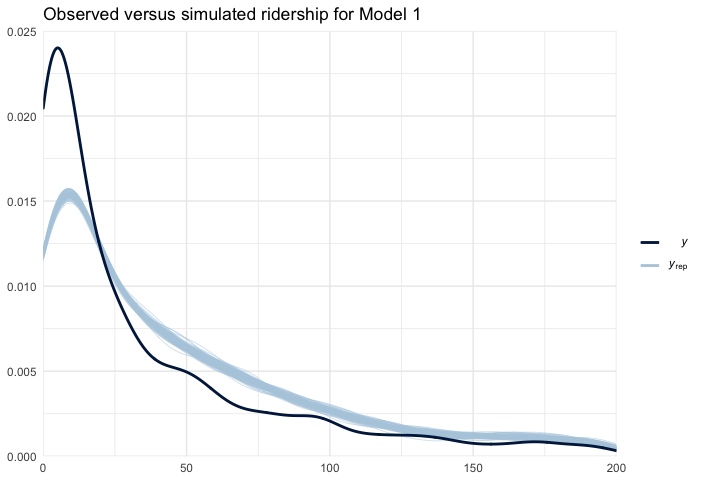
\includegraphics[width = 6in]{ppcheck_mod1.png}
  \caption{Posterior predictive check for Model 1.}
\end{figure}

Model 1 clearly underestimates the number of block groups with low
ridership. This is due in large part to extra-Poisson variance present
in Metro Transit's ridership data.

\hypertarget{overdispersed-poisson-regression}{%
\subsection{Overdispersed Poisson
Regression}\label{overdispersed-poisson-regression}}

The most obvious assumption made in a Poisson regression is that
response variable \(Y\) follows a Poisson distribution. In addition to
requiring integer counts, this assumption requires that
\(\text{Var}(Y) = \text{E}(Y)\). This is often not true in practice. In
the case of the Metro Transit ridership data,
\(\text{Var}(Y) >>\text{E}(Y)\). In this case, we call the unexpectedly
large variance ``overdispersion'' or ``extra-Poisson variance.''

Data with this feature can be difficult to model directly with a Poisson
regression. One option is to use a generalization of the Poisson
distribution, such as a Negative-Binomial distribution, as the
observation model. For the Metro Transit application, we instead modify
the latent function to include a seperate term to account for
overdispersion. As such, the Poisson regression above can be rewritten
to include

\[
\begin{aligned}
\eta_i = log(\lambda_i) & = \beta_0 + \sum_{k=1}^{K}x_k^T\beta_k + \theta\sigma \\
\theta &\sim \text{Normal}(0, 1) \\
\sigma &\sim \text{Normal}(0, 5)
\end{aligned}
\]

where \(\theta\) is a set of heterogenous random effects. In practice,
\(\theta\) is scaled by its variance parameter \(\sigma\) to allow
eassier fitting in Stan. The addition of this set of random effects
improves fits on data with overdispersion. With sufficiently vague
priors, \(\theta\) and \(\sigma\) can account for most or all of the
overdispersion not accounted for by
\(\beta_0 + \sum_{k=1}^{K}x_k^T\beta_k\).

\hypertarget{model-2}{%
\subsubsection{Model 2}\label{model-2}}

Model 2 builds upon Model 1 by incorporating the set of random effects
described above. Model 2 is \emph{significantly} more computationally
expensive to fit than Model 1. This is due to relatively large
autocorrelation between each iteration, visible in the traceplots below
(Figure \_\_\_). This autocorrelation made it necessary to run Model 2
on four chains for 20,000 iterations each. Despite this, \texttt{n\_eff}
is significantly lower for Model 2 than Model 1. Model 2 also
experienced 2 transitions exceeding maixmum treedepth: not a problem in
terms of model fit, but a signal that the posterior is more challenging
to fit. Reparameterization could likely reduce autocorrelation between
iterations.

The parameter estimates for \(\beta_0\) and \(\beta\) for Model 2 are
below. Notably, the direction and magnitude of the coefficient estimates
are similar to those produced by Model 1. However, the coverage
intervals are much wider. Based on ``test runs'' of Model 2, we expect
increasing the number of iterations to decrease the width of these
coverage intervals (we observe that the converage interval is
proportional to the number of iterations in this setting).

\begin{table}[H]
\centering
\begin{tabular}{lrrrrrr}
  \toprule
Parameter & Rhat & n\_eff & mean & sd & 2.5\% & 97.5\% \\ 
  \midrule
beta\_0 & 1.0 & 1354 & -1.9 & 0.0 & -2.0 & -1.8 \\ 
  sigma & 1.0 & 1800 & 1.0 & 0.0 & 0.9 & 1.0 \\ 
  beta[1] & 1.0 & 1546 & -0.1 & 0.0 & -0.2 & -0.0 \\ 
  beta[2] & 1.0 & 1095 & 0.0 & 0.1 & -0.1 & 0.1 \\ 
  beta[3] & 1.0 & 1322 & 0.0 & 0.0 & -0.0 & 0.1 \\ 
  beta[4] & 1.0 & 1208 & -0.0 & 0.0 & -0.1 & 0.0 \\ 
  beta[5] & 1.0 & 1282 & -0.0 & 0.0 & -0.1 & 0.1 \\ 
  beta[6] & 1.0 & 988 & 0.1 & 0.0 & 0.1 & 0.2 \\ 
  beta[7] & 1.0 & 1019 & 0.1 & 0.0 & -0.0 & 0.1 \\ 
  beta[8] & 1.0 & 1178 & 0.0 & 0.0 & -0.0 & 0.1 \\ 
  beta[9] & 1.0 & 1125 & 0.0 & 0.0 & -0.1 & 0.1 \\ 
  beta[10] & 1.0 & 1796 & 0.1 & 0.0 & 0.1 & 0.2 \\ 
  beta[11] & 1.0 & 1152 & -0.1 & 0.0 & -0.1 & -0.0 \\ 
  beta[12] & 1.0 & 1629 & 0.0 & 0.0 & -0.0 & 0.1 \\ 
  beta[13] & 1.0 & 2101 & -0.0 & 0.0 & -0.1 & 0.0 \\ 
  beta[14] & 1.0 & 1415 & -0.1 & 0.0 & -0.1 & -0.0 \\ 
  beta[15] & 1.0 & 1581 & 0.1 & 0.0 & 0.0 & 0.2 \\ 
  beta[16] & 1.0 & 1160 & -0.1 & 0.0 & -0.2 & -0.0 \\ 
  beta[17] & 1.0 & 997 & 0.1 & 0.0 & 0.0 & 0.2 \\ 
  beta[18] & 1.0 & 1589 & -0.0 & 0.0 & -0.1 & 0.0 \\ 
   \bottomrule
\end{tabular}
\caption{Stan output for Model 2} 
\end{table}

\begin{figure}[H]
  \centering
  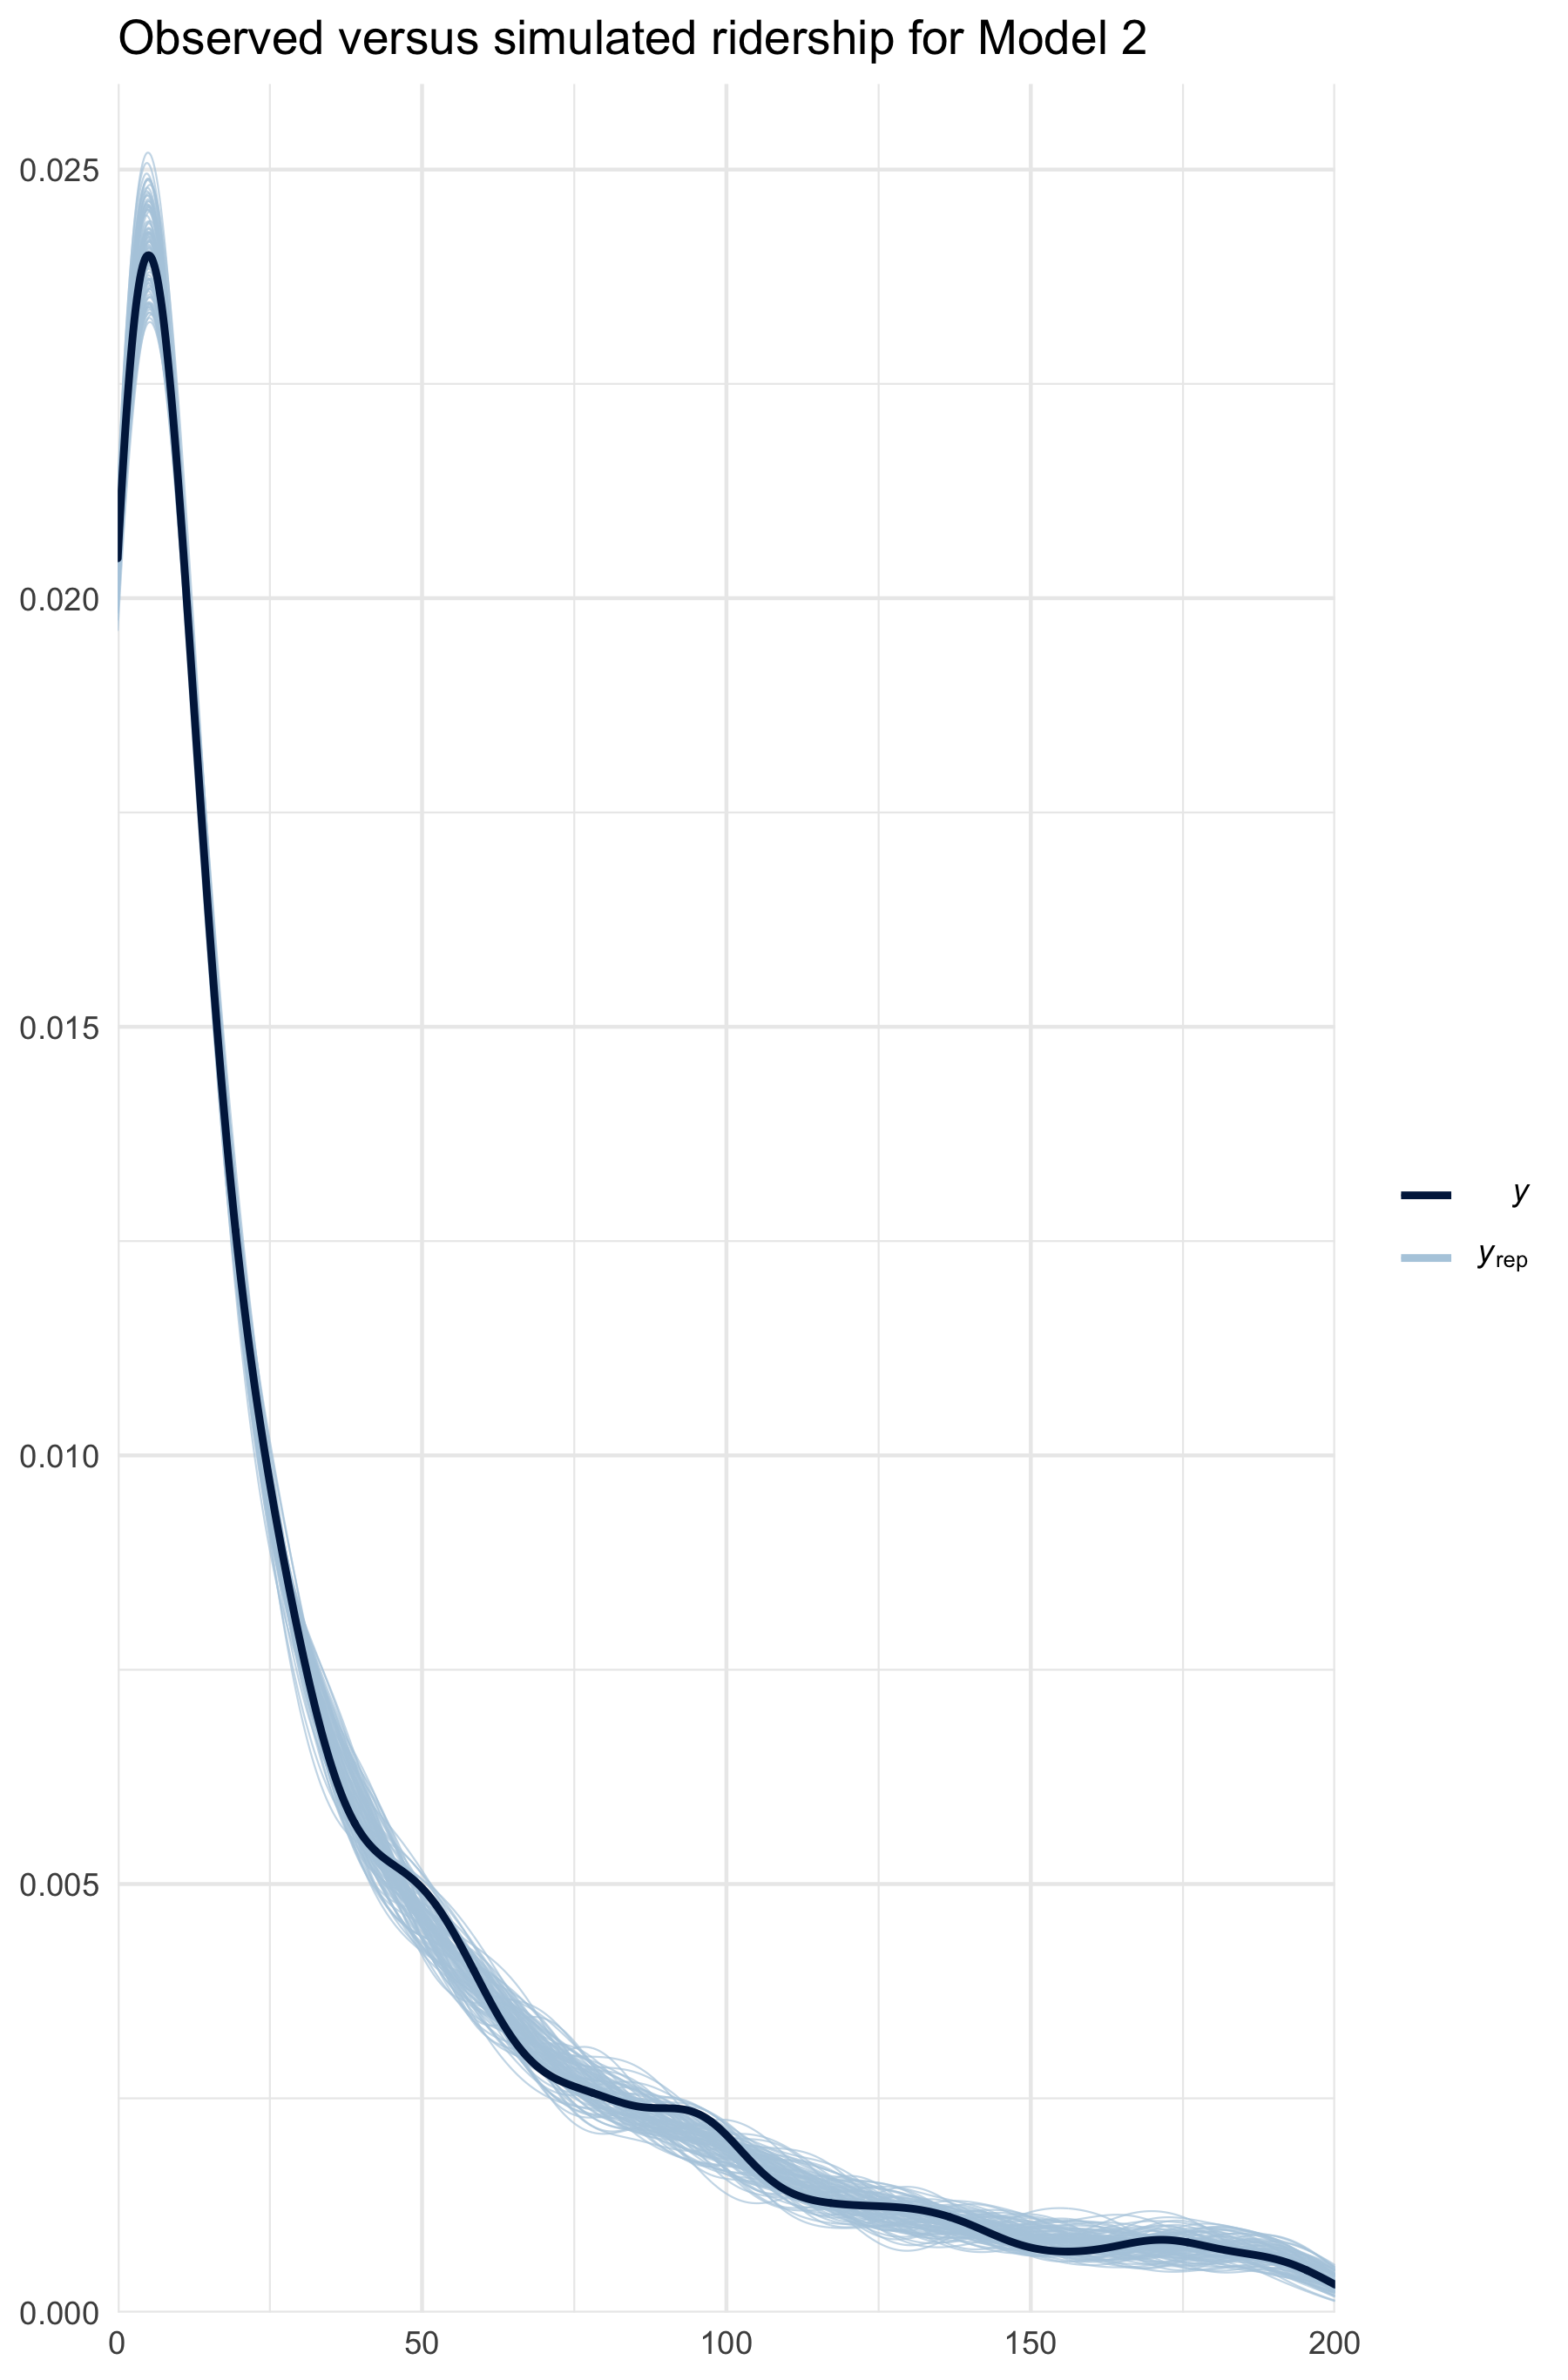
\includegraphics[width = 6in]{ppcheckmod2.png}
  \caption{Posterior predictive check for Model 1.}
\end{figure}

Because we gave \(\theta\) and \(\sigma\) vague priors, we can see a
\emph{much} better fit in the posterior predictive checks for Model 2.
One \emph{could} stop analysis here. However, the addition of
\(\theta \sigma\) only improves the \emph{fit} of the model, not our
understanding of the data. Therefore, for this study, we will decompose
\(\theta \sigma\) into spatial and non-spatial random effects. First,
however, we will implement a Bayesian variable selection process to
determine which, if any, of our covariates \(x_k\) should be removed
from the analysis.

\hypertarget{horseshoe-priors-and-variable-selection}{%
\subsection{Horseshoe Priors and Variable
Selection}\label{horseshoe-priors-and-variable-selection}}

In the baseline model, we give coefficients \(\beta_1, ..., \beta_k\)
simple normal priors. With a large set of possible covariates, however,
we may reasonably expect some of the \(\beta_k\) coefficients to be
equal to zero -- in other words, that some of the parameters \(x_k\)
have no effect on response \(Y\). In frequentist applications, we might
use a method such as the LASSO (Least Absolute Shrinkage and Selection
Operator) to identify relevant variables. There are several Bayesian
alternatives for variable selection with generally consist of applying
particular priors to \(\beta\).

\hypertarget{spike-and-slab---needs-graphics}{%
\subsubsection{Spike and Slab - needs
graphics}\label{spike-and-slab---needs-graphics}}

In the Bayesian setting, there are two primary methods for variable
selection. The first is called the ``spike-and-slab'' prior (Mitchell
and Beauchamp, 1988; George and McCulloch, 1999) and has often been
considered the ``gold standard'' for sparse Bayesian regression, or
variable selection (Piironen and Vehtari, 2017). This prior is often
expressed as

\[
\begin{aligned}
\beta_j | \lambda_j, c, \epsilon & \sim \lambda_j \text{Normal}(0, c^2) + (1-\lambda_j)\text{Normal}(0, \epsilon^2) \\
\lambda_j & \sim \text{Bernoulli}(\pi)
\end{aligned}
\]

for \(j = 1, 2, ..., J\) where \(\lambda_j \in {0, 1}\) indicates
whether \(\beta_j\) is from the ``spike'' (ie, near zero) or the
``slab'' (ie, nonzero). The ``spike'' is the area where most of the
prior density for \(\beta\) is centered (generally around 0) while the
``slab'' refers to the low-density extent of the prior. The
spike-and-slab prior encourages all \(\beta_j\) towards zero; only
\(\beta_j\) sufficiently far from 0 will be estimated to be from the
slab.

The primary challenge with the spike-and-slab (and other Bayesian
shrinkage methods) is the selction of priors. Priors must be set for the
width of the slab \(c\) and the prior inclusion probability \(\pi\).
Here, \(\pi\) reflects our prior understanding of the sparsity of
\(\beta\). In practice, we rarely have strong prior knowledge of the
number of predictors we expect to be distinguishable from zero. This can
make the implementation of sparse regression more challenging than, say,
the frequentist LASSO.

\hypertarget{horseshoe---needs-graphics}{%
\subsubsection{Horseshoe - needs
graphics}\label{horseshoe---needs-graphics}}

The second method for Bayesian sparse regression is to give \(\beta\)
some continuous \emph{sparsity inducing prior}. \textbf{Van Erp et al
(2019)} provide an introduction to many such continous priors. Ridge
regression and the Bayesian LASSO are two of the most approachable
priors, but all sparsity inducing priors utilize the same logic as the
spike-and-slab: give \(\beta\) a prior with \emph{most} of its mass near
0, to shrink irrelevant coefficients, and the rest of its mass ``far''
from 0. Identifying ``far'' depends more or less on the specific data
and model in question.

The horseshoe prior, proposed by \textbf{Carvalho et al, 2010} is a
popular choice in Bayesian literature, in part because it is similar to
the ``gold standard'' spike-and-slab. Following the notation of
\textbf{Vehtari \& Piironen}, the horseshoe prior can be expressed

\[
\begin{aligned}
\beta_k \text{ | } \lambda_k, \tau & \sim \text{Normal}(0, \tau^2\lambda_k^2) \\
\lambda_k & \sim \text{Half-Cauchy}(0, 1)
\end{aligned}
\]

for \(k = 1, 2, ..., K\). The horseshoe prior is so-named because for
fixed values \(\tau = \lambda_k = 1\), the prior resemebles a Beta(1/2,
1/2) distribution, or a horseshoe.

The horseshoe is often favored because it is a global-local shrinkage
prior. This means that \(\tau\) shrinks \emph{all} parameters towards 0
while the local parameter \(\lambda_k\) and the heavy Cauchy tails allow
larger coefficients to remain unshrunk. While this is precisely the goal
of a sparsity inducing prior, the horseshoe prior can fail to regularize
large coefficients \emph{at all}, which can be a problem when parameters
are weakly identified by data. With no regularization applied to the
largest coefficients, there is a risk of overfitting. Additionally,
there is no consensus in the literature for assigning priors to \(tau\).
Piironen and Vehtari (2017) introduced the \emph{regularized horseshoe}
to address both of these shortcomings of the horseshoe.

\hypertarget{regularized-horseshoe---needs-graphics}{%
\subsubsection{Regularized Horseshoe - needs
graphics}\label{regularized-horseshoe---needs-graphics}}

The regularized horseshoe builds upon the horseshoe prior such that

\[
\begin{aligned}
\beta_k \text{ | } \lambda_j, \tau, c & \sim \text{Normal}(0, \tau^2 \tilde{\lambda_k^2}) \\
\tilde{\lambda_k^2} & = \frac{c^2\lambda_k^2}{c^2 + \tau^2\lambda_k^2} \\
\lambda_k & \sim \text{Half-Cauchy}(0, 1) \\
c & \sim ~ \text{Inverse-Gamma}(a, b) \\
\tau & \sim 
\end{aligned}
\]

where \(c\) \textgreater{} 0 helps to regularize \(\beta_k\) far from
zero. When \(c\) approaches infinity, the regularized horseshoe becomes
the standard horseshoe. Additionally, \(c\) in the regularized horseshoe
corresponds to the slab width in the spike-and-slab prior.

As with the spike-and-slab, the selection of priors is a challenge with
the regularized horseshoe. Piironen and Vehtari (2017) provide a set of
recommendations for setting priors which we follow in this study. In
practice, we tune the priors for \(\lambda_k\), \(c\), and \(\tau\)
using simulated data with features similar to our observed data (ie,
parameters with coefficients of similar magnitude).

\hypertarget{model-3}{%
\subsubsection{Model 3}\label{model-3}}

For this study, we implement the regularized horseshoe using code
modified from Piironen \& Vehtari.

Notably, Model 3 experienced one divergent transition after warmup.
However, the model was fitted several times with no divergent
transitions. A ``false alarm'' divergent transition can occur when the
cutoff for determining a divergent transition is too low; this can be
true in the case of particularly complex posteriors. Because only 1 out
of 20,000 iterations produced a divergent transition, we can proceed
with caution using Model 3. Additionally, the parameter estimates
provided by Model 3 closely match those from Models 1 and 2, suggesting
that the single divergent transition did not have an adverse effect on
the posterior estimates.

The posterior predictive checks for Model 3 match Model 2 almost
perfectly - this is to be expected. The addition of horseshoe priors on
\(\beta_k\) does not attempt to improve model fit, but to determine
which covariates are most ``important''.

On that note, we can see that Model 3 \emph{did} shrink two \(\beta_k\)
exactly to zero.

\hypertarget{adding-spatial-structure}{%
\subsection{Adding Spatial Structure}\label{adding-spatial-structure}}

When modeling data with a spatial component, we generally expect
adjacent areas to be more similar than areas which are far apart. While
this is a straightforward assumption, it can improve model fits in
several ways. First, it can encode prior information about response
\(Y\) not otherwise represented by covariates \(x\) (ie, that nearby
observations are more similar than far-flung ones). Second, it can
provide geographic smoothing when observations are sparse or noisy. This
is often the case in small areas or when observing events which can only
occur at specific locations, such as air quality measured by sensors. In
the case of the Metro Transit ridership data, this smoothing can help
avoid overfitting areas such as the outliers in downtown Minneapolis and
better represent block groups with no existing bus stops.

In the case of Metro Transit's ridership data, we expect encoding
spatial structure to improve the model fit in several ways. First, we
know that assigning transit ridership to census geography is inherently
flawed. This is because census geographies, including block groups, are
generally bounded by major roads (in addition to natural features such
as lakes and political boundaries such as city limits). Naturally, bus
stops tend to exist along those same major roadways.

This bounding convention means that boardings are often assigned to
different block groups depending on which direction the passenger is
travelling. For example, consider the A-Line running along Snelling
Avenue. Boarding at Snelling and Grand \emph{northbound} puts you in
block group \_\_\_\_ while boarding at the same intersection but
\emph{southbound} puts you in block group \_\_\_\_. Integrating spatial
structure will help to smooth ridership across block group bounds.
\textbf{will add a map here}

Additionally, we know intuitively that transit riders don't necessarily
board in the block groups they live in. Particularly in dense areas,
it's very likely for riders to board in a block group other than the
block group they reside in. For example, I live in block group \_\_\_\_
but walk about 10 minutes to board the A-Line southbound at Snelling and
Randolph. Commuting patterns such as these can assign ridership to
different block groups than we might expect. Geographic smoothing will
allow neighboring block groups to share information, better representing
these ridership patterns.

\hypertarget{conditional-autoregressive-priors}{%
\subsubsection{Conditional Autoregressive
Priors}\label{conditional-autoregressive-priors}}

Conditional Autoregressive (CAR) priors are one of the most widespread
Bfayesian methods for modeling spatial autocorrelation. CAR models were
introduced in Besag 1974 and remain perhaps the primary method for
Bayesian areal data modeling. Note that CAR models are recommended for
use as \emph{priors} rather than as an observation model.

Areal data corresponds to finitely many discrete areal units, such as
counties or census tracts. CAR priors are often used in the context of
small-area count data. This sort of response variable tends to be noisy,
particularly when the counted event is rare, the population of areal
unit \(i\) is small, or the physical boundaries of areal units present
challenges. CAR priors were designed in part to smooth such noisy
counts. As such, they are often applied in epidemiological disease risk
modeling in which disease occurences may be rare.

Generally, CAR models rely on a binary neighborhood structure. Areal
units \(i\) and \(j\) are considered neighbors if they share a boundary.
For strictly rectangular lattice data, we often choose either a
``Queens'' or ``Rooks'' neighborood structure. \textbf{insert graphics}
For irregularly shaped areal data, such as our 1,495 census block
groups, we generally default to a queen neighborhood structure wherein
areal units sharing \emph{any} points of contact are deemed neighbors.

For \(n\) regions, the neighorhood relationships are encoded in an
\(n \times n\) neighborhood matrix \(W\). Matrix \(W\) is defined such
that \(w_{ij} = 1\) if if regions \(i\) and \(j\) are neighbors (denoted
\(i \sim j\)) and 0 otherwise. This matrix is symmetric. Note that
regions are not considered neighbors of themselves, ie the diagonal
entries \(w_{ii} = 0\).

The spatial interactions are modeled by a random variable \(\phi\).
Here, \(\phi\) is a vector \(\phi = \phi_1, \phi_2, ..., \phi_n\). The
distribution of each \(\phi\) is determined by the sum of its neighbors'
values such that

\[
\phi_i \text{ | } \phi_j, j \neq i \sim \text{Normal}(\sum_{i=1}^{N}w_{ij}\phi_j, \sigma^2) 
\]

The conditional distribution of each \(\phi_i\) is helpful in building
intuition about the functionality of the CAR prior. Basing the value of
each \(\phi_i\) off of its neighbors is how the CAR prior performs
spatial smoothing.

Besag (1974) proved that the joint distribution of \(\phi\) is a
multivariate normal centered at 0 where its variance is given by a
symmetric positive definite precision matrix \(Q\). Matrix \(Q\) is
simply the inverse of the covariance matrix \(\sum\). This finding
simplifies the above to

\[
\phi \sim \text{Normal}(0, Q^{-1})
\]

Precision matrix \(Q\) can be defined for multivariate normal \(\phi\)
using two other \(n \times n\) matrices: the neighborhood matrix \(W\)
and the diagonal matrix \(D\) in which \(d_{ii}\) indicates the number
of neighbors region \(i\) has. All off-diagonal entries are 0. Using
these matrices, \(Q\) is defined

\[
Q = D(I - \alpha W)
\]

where \(I\) is the identity matrix and \(\alpha \in (0, 1)\) determines
the amount of spatial autocorrelation present in \(Y\). Parameter
\(\alpha\) is a key component of CAR models. At \(\alpha = 0\), the
model assumes spatial independence and at \(\alpha = 1\), perfect
spatial autocorrelation.

Following Morris et al, the log probability density of \(\phi\) is
proportional to

\[
\frac{M}{2}\text{log(det}(Q)) - \frac{1}{2}\phi^TQ\phi
\]

Calculating this value is computationally expensive. For models with
1,000 areal units, for example, calculating the determinant requires 1
billion operations (Morris et al, 2019). Given that the Metro Transit
ridership data corresponds to 1,495 areal units, a strict CAR prior may
be too computationally inefficient for our models.

\hypertarget{intrinsic-conditional-autoregressive}{%
\subsubsection{Intrinsic Conditional
Autoregressive}\label{intrinsic-conditional-autoregressive}}

The Intrinsic Conditional Autoregressive (ICAR) prior is a slight
simplifation of a CAR prior. ICAR priors set \(\alpha = 1\) which
simplifies the definition of Q

\[
Q = D-A
\]

thereby setting \(det(Q) = 0\). As a result, the first term in
**equation \_\_\_** can be simplified to

\[
-\frac{1}{2}\phi^TQ\phi
\]

This reduces the computational expense of computing CAR models
significantly. Notably, the ICAR prior is improper but yields proper
posteriors (Morris et al, 2019).

The ICAR prior specifies each \(\phi_i\) to be normally distributed with
its mean equal to the mean of its neighbor's values. This is how the
CAR/ICAR model ``borrows strength'' from geographic neighbors to smooth
noisy estimates. Intuitively, the variance of each \(\phi_i\) decreases
as its number of neighbors \(d_i\) increases. The conditional
distribution for each \(\phi_i\) can be written

\[
\text{p}(\phi_i \text{ | } \phi_{i \sim j}) = \text{Normal}(\frac{\sum_{i \sim j}\phi_i}{d_i}, \frac{\sigma_i^2}{d_i})
\]

Here, the variance \(\sigma\) is unknown. The conditional specification
of each \(\phi_i\) is helpful in building intuition about the
assumptions the ICAR component makes and how it performs its
``smoothing''. The ICAR prior matches our intuition about spatial
autocorrelation: areal unit \(i\) is similar to the areal units
surrounding it, and the more areal units surround it, the more confident
we feel in that similarity. The joint distribution can be rewritten

\[
\text{p}(\phi) \propto \text{exp}(-\frac{1}{2}\sum_{i \sim j}(\phi_i - \phi_j)^2)
\]

This pairwise difference specification is more computationally efficient
to fit in Stan (Morris et al, 2019).

\hypertarget{besag-york-mollie-bym}{%
\subsubsection{Besag-York-Mollie (BYM)}\label{besag-york-mollie-bym}}

The specific ICAR model used in this analysis is the Besag-York-Mollie
(BYM) Poisson model. The BYM is a ``classical'' spatial Bayesian method
(Riebler et al, 2016). It is generally used in disease mapping studies
to model rare events (ie, disease occurrence) in small areal units. The
BYM capitalizes on the ICAR prior's ability to smooth noisy estimates
and share information across geographic units.

The latent function in the BYM model contains heterogeneous random
effects as well as a spatial ICAR term in order to account for both
spatial and non-spatial heterogeneity. Note that in Section \_\_\_, we
introduced a random effect term \(\theta\). Therefore, the BYM model can
be though of as decomposing \(\theta\) into spatial and non-spatial
components.

Specifically, the BYM model replaces \(\eta_i\) from equation \_\_\_
with

\[
\eta_i = \beta_0 + \sum_{k=1}^{K}x_k^T\beta_k + \theta + \phi
\]

where \(\phi\) is the addition: an ICAR component. Decomposing
overdispersion as such is helpful in furthering our understanding of
response \(Y\). When we use a simple random effect \(\theta\) alone, we
can accomplish a good model fit. However, \(\theta\) provides no
additional information about \(Y\). The decomposition of \(\theta\) in
the BYM allows us to better quantify how much variance is white noise
(ordinary random effects) versus some unmeasured confounding correlated
across space.

The BYM model as written above is appealing in its simplicity. However,
the lack of informative hyperpriors specified for \(\theta\) and
\(\phi\) can make the model incredibly challenging to fit. In theory,
extra-Poisson variance could be explained 100\% by \(\theta\), 100\% by
\(\phi\), or anywhere in between. In \emph{practice}, we likely have
limited information about where that ratio falls. Riebler et al (2016)
further explain the sampling issues faced by the BYM model faced with no
hyperpriors. In short, the sampler is forced to explore all possible
combinations of \(\theta\) and \(\phi\), no matter how unlikely a
particular combination my be. In the context of fitting models with
Stan, this is liekly to cause uneccesarily long computation times and
perhaps to yield biased posterior estimates.

There are some suggestions in the literature for setting hyperpriors for
\(\theta\) and \(\phi\) (Besag and Mollie, 1991; Clayton and Montomoli,
1995). The existing methods, however, tend to rely on the specific data
at hand which makes the selection of hyperparameters unnecessarily time
consuming.

\hypertarget{bym2}{%
\subsubsection{BYM2}\label{bym2}}

The BYM2 model proposed by Simpson et al and further described in
Riebler et al (2016) aims to solve these sampling problems. The BYM2
takes a more ``fully Bayesian'' approach to hyperprior/hyperparameter
selection. The primary difference between the BYM and BYM2 models is the
addition of a mixing parameter, \(\rho\). The BYM2 model rewrites the
BYM as

\[
\eta_i = \beta_0 + \sum_{k=1}^{K}x_k^T\beta_k + ((\sqrt{\frac{\rho}{s}})\theta^{*} + ((\sqrt{1-\rho})\phi^{*})\sigma
\]

where \(\rho \in (0, 1)\) determines how much variance/overdispersion is
caused by spatial versus non-spatial error terms. Like the popular
Leroux CAR prior, proposed by Leroux et al (2009), the BYM2 scales both
\(\theta\) and \(\phi\) by \(\sigma\), the standard deviation of the
combined error terms (Morris et al, 2019). In this parameterization,
\(s\) is a scaling factor such that Var(\(\theta_i\)) \(\approx\)
Var(\(\phi_i\)) \(\approx\) 1. The equal unit variance is necessary for
\(\sigma\) to truly be the standard deviation of the error terms.

Setting priors is somewhat more straightforward for the BYM2. The ICAR
component, \(\phi^{*}\) remains unchanged. Riebler and Morris recommend
the prior \(\theta \sim\) Normal(\(0, n)\) where \(n\) is the number of
connected graphs in the neighborhood graph. In many cases, such as
modeling data for all counties in a state, \(n=1\). When \(n>1\), the
variance is different in each subgraph which affects \(\sigma\) and
\(s\). It is possible to fit the model in this case, although
computation time is much longer.

A relatively vague Normal(0, 1) prior is appropriate for \(\sigma\).
Riebler et al (2016) also propose either a Beta(1/2, 1/2) or more
specialized, complex prior for mixing parameter \(\rho\). For this
study, we use the simpler Beta(1/2, 1/2) prior.

\hypertarget{model-4}{%
\subsubsection{Model 4}\label{model-4}}

Model 4 uses all 18 covariates of interest, no horseshoe priors, and
decomposes \(\theta\sigma\) into a set of random effects plus a spatial
ICAR component. This model converges much more efficiently than Model 2
or Model 3 due to careful reparameterization of the BYM by Riebler et al
(2016). Future would could potentially improve the speed of fitting
Models 2 and 3.

Model 4 was run on four chains for 10,000 iterations each. The parameter
estimates for Model 4 are below. Note that \texttt{n\_eff} is lower than
for Model 1 but significantly higher than Model 2 or 3.

\begin{table}[ht]
\centering
\begin{tabular}{lrrrrrr}
  \toprule
Parameter & Rhat & n\_eff & mean & sd & 2.5\% & 97.5\% \\ 
  \midrule
beta0 & 1.001 & 4770 & -1.880 & 0.028 & -1.937 & -1.825 \\ 
  sigma & 1.003 &  520 & 2.698 & 0.372 & 1.993 & 3.451 \\ 
  rho & 1.002 &  514 & 0.888 & 0.038 & 0.793 & 0.941 \\ 
  theta[5] & 1.000 & 17797 & -0.179 & 0.777 & -1.688 & 1.336 \\ 
  beta[1] & 1.000 & 4322 & 0.034 & 0.047 & -0.056 & 0.127 \\ 
  beta[2] & 1.001 & 3801 & 0.061 & 0.035 & -0.009 & 0.131 \\ 
  beta[3] & 1.000 & 4203 & -0.003 & 0.039 & -0.080 & 0.073 \\ 
  beta[4] & 1.001 & 4330 & -0.049 & 0.044 & -0.134 & 0.037 \\ 
  beta[5] & 1.000 & 4706 & 0.209 & 0.042 & 0.127 & 0.292 \\ 
  beta[6] & 1.000 & 4919 & 0.065 & 0.038 & -0.009 & 0.138 \\ 
  beta[7] & 1.002 & 3929 & 0.029 & 0.038 & -0.046 & 0.104 \\ 
  beta[8] & 1.000 & 6278 & 0.145 & 0.032 & 0.083 & 0.207 \\ 
  beta[9] & 1.000 & 4607 & -0.088 & 0.031 & -0.150 & -0.026 \\ 
  beta[10] & 1.000 & 6145 & 0.014 & 0.029 & -0.043 & 0.070 \\ 
  beta[11] & 1.000 & 6978 & -0.022 & 0.031 & -0.083 & 0.040 \\ 
  beta[12] & 1.000 & 6125 & -0.068 & 0.034 & -0.136 & -0.002 \\ 
  beta[13] & 1.000 & 5875 & 0.094 & 0.033 & 0.029 & 0.158 \\ 
  beta[14] & 1.000 & 4743 & -0.089 & 0.035 & -0.157 & -0.019 \\ 
  beta[15] & 1.001 & 2720 & 0.076 & 0.039 & 0.001 & 0.151 \\ 
  beta[16] & 1.000 & 6053 & -0.029 & 0.031 & -0.091 & 0.031 \\ 
   \bottomrule
\end{tabular}
\caption{Stan output for Model 4} 
\end{table}

Like Models 2 and 3, the BYM2 model performs well in the posterior
predictive check (Figure \_\_).

\begin{figure}[H]
  \centering
  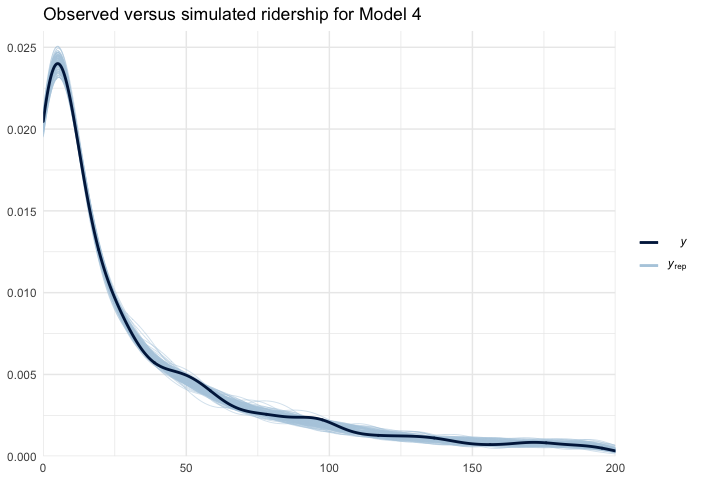
\includegraphics[width = 6in]{ppcheckmod4.png}
  \caption{Posterior predictive check for Model 1.}
\end{figure}

\hypertarget{model-5}{%
\subsubsection{Model 5}\label{model-5}}

Model 5 builds upon Model 4 by incorporating regularized horsehoe priors
in addition to spatial ICAR priors. This model has high autocorrelation
between iterations and took \emph{significantly} longer than any of the
other models to fit in Stan (upwards of 12 hours). That said, the
\texttt{n\_eff} and \(\hat{R}\) diagnostics indicate convergence and the
parameter estimates (Table \_\_) match our expectations in terms of sign
and magnitude based on the previous 4 models.

\begin{table}[H]
\centering
\begin{tabular}{lrrrrrr}
  \toprule
Parameter & Rhat & n\_eff & mean & sd & 2.5\% & 97.5\% \\ 
  \midrule
beta0 & 1.000 & 5837 & -1.878 & 0.028 & -1.934 & -1.822 \\ 
  sigma & 1.010 &  721 & 2.826 & 0.359 & 2.138 & 3.561 \\ 
  theta[5] & 1.000 & 19566 & -0.188 & 0.787 & -1.722 & 1.349 \\ 
  rho & 1.012 &  713 & 0.900 & 0.031 & 0.824 & 0.946 \\ 
  phi[5] & 1.004 & 1652 & 5.974 & 1.573 & 3.264 & 9.527 \\ 
  beta[1] & 1.001 & 3637 & -0.119 & 0.059 & -0.233 & -0.002 \\ 
  beta[2] & 1.001 & 8170 & -0.005 & 0.027 & -0.069 & 0.049 \\ 
  beta[3] & 1.000 & 3987 & 0.024 & 0.030 & -0.019 & 0.096 \\ 
  beta[4] & 1.000 & 8531 & -0.004 & 0.022 & -0.057 & 0.040 \\ 
  beta[5] & 1.000 & 7619 & -0.012 & 0.026 & -0.076 & 0.030 \\ 
  beta[6] & 1.001 & 2999 & 0.164 & 0.055 & 0.051 & 0.268 \\ 
  beta[7] & 1.000 & 3726 & 0.032 & 0.035 & -0.016 & 0.114 \\ 
  beta[8] & 1.000 & 7956 & 0.010 & 0.025 & -0.032 & 0.074 \\ 
  beta[9] & 1.000 & 5622 & 0.019 & 0.028 & -0.023 & 0.089 \\ 
  beta[10] & 1.000 & 7530 & 0.144 & 0.033 & 0.079 & 0.208 \\ 
  beta[11] & 1.000 & 4558 & -0.057 & 0.034 & -0.123 & 0.001 \\ 
  beta[12] & 1.000 & 11150 & 0.004 & 0.018 & -0.031 & 0.046 \\ 
  beta[13] & 1.000 & 8289 & -0.017 & 0.024 & -0.073 & 0.020 \\ 
  beta[14] & 1.000 & 5469 & -0.028 & 0.031 & -0.100 & 0.015 \\ 
  beta[15] & 1.000 & 4822 & 0.060 & 0.035 & -0.001 & 0.130 \\ 
  beta[16] & 1.001 & 3863 & -0.060 & 0.038 & -0.134 & 0.003 \\ 
  beta[17] & 1.000 & 2094 & 0.051 & 0.041 & -0.008 & 0.137 \\ 
  beta[18] & 1.000 & 6949 & -0.010 & 0.021 & -0.061 & 0.026 \\ 
   \bottomrule
\end{tabular}
\caption{Stan output for Model 5} 
\end{table}

The posterior predictive checks and mapped residuals for Model 5 are
very similar to those for Model 4. Like Model 2, the slow sampling time
is largely caused by autocorrelation between iterations.

The more interesting comparison here is with Model 3. The horseshoe
priors in Model 5 fail to shrink any parameters \emph{exactly} to zero.
As previously discussed, running the model for more iterations would
likely cuase the coverage intervals on the \(\beta_k\) estimates to
tighten.

\hypertarget{discussion}{%
\section{Discussion}\label{discussion}}

In this study, we fit several increasingly complex models building upon
the baseline Poisson regression, Model 1. Model 2 incorporates a simple
set of random effects to account for overdispersion. Model 3
incorporates regularized horseshoe priors for variable selection. Model
4 includes the spatial ICAR priors but no horseshoe priors, and Model 5
includes both regularized horseshoe priors and ICAR priors.

All five models were run for at least 10,000 iterations and ``pass'' the
basic diagnostic checks: \(\hat{R} = 1\), sufficiently high
\texttt{n\_eff}, and no concerning \texttt{max\_treedepth} or divergence
warnings.

Naturally, the baseline Model 1 converges most quickly and has the
highest \texttt{n\_eff} diagnostics. The simplicity of the Model,
however, yields a poor model fit. Perhaps unexpectedly, Model 4, the
BYM2, is the second-most efficient in terms of convergence and Effective
Sample Size.

While the most complex model \emph{does} converge and provide reasonable
parameter estimates, its computational inefficiency may not be worth the
addition of horseshoe priors to the BYM2 model, depending on the
application. A more efficient approach may be to conduct variable
selection using horseshoe priors on a simpler model (in our case, Model
1 or Model 3, for example) before incorporating the ICAR component.

\hypertarget{appendix-stan-code}{%
\section{Appendix: Stan Code}\label{appendix-stan-code}}

\hypertarget{model-1-1}{%
\subsection{Model 1}\label{model-1-1}}

The Stan program for the baseline model is below. This model could also
have been fit using Stan's more efficient built-in Poisson GLM function.
For this study, we write the GLM more ``longhand'' for ease of
comparison between models.

\begin{verbatim}
## data {
##   // number obs
##   int<lower=0> N;
##   // response
##   int<lower=0> y[N];       
##   // "offset" (number of stops)
##   vector<lower=0>[N] E;     
##   // number of covariates
##   int<lower=1> K;
##   // covariates
##   matrix[N, K] x;
## }
## transformed data {
##   vector[N] log_E = log(E);
## }
## parameters {
##   // intercept
##   real beta_0;      
##   // covariates
##   vector[K] beta;          
## }
## transformed parameters{
##   // latent function variables
##   vector[N] f;
##   f = log_E + beta_0 + x*beta;
## }
## model {
##   /// model 
##   y ~ poisson_log(f); 
##   // prior on betas
##   beta_0 ~ normal(0.0, 3);
##   beta ~ normal(0.0, 1);
## }
## generated quantities {
##   vector[N] log_lik; 
##     for(i in 1:N) log_lik[i] = poisson_log_lpmf(y[i] | log_E[i] + beta_0 + x[i,]*beta);
## }
\end{verbatim}

\hypertarget{model-2-1}{%
\subsection{Model 2}\label{model-2-1}}

The Stan program for Model 2 differs from Model 1 only in the latent
variable, \texttt{f}.

\begin{verbatim}
## data {
##   // number obs
##   int<lower=0> N;
##   // response
##   int<lower=0> y[N];       
##   // "offset" (number of stops)
##   vector<lower=0>[N] E;     
##   // number of covariates
##   int<lower=1> K;
##   // covariates
##   matrix[N, K] x;
## }
## transformed data {
##   vector[N] log_E = log(E);
## }
## parameters {
##   // intercept
##   real beta_0;      
##   // covariates
##   vector[K] beta;   
##   // overdispersion
##   vector[N] theta;
##   // random effects variance
##   real<lower=0> sigma;
## }
## transformed parameters{
##   // latent function variables
##   vector[N] re; 
##   vector[N] f;
##   re = theta * sigma; 
##   f = log_E + beta_0 + x*beta + re;
## }
## model {
##   /// model 
##   y ~ poisson_log(f); 
##   // prior on betas
##   beta_0 ~ normal(0.0, 1);
##   beta ~ normal(0.0, 0.2);
##   // overdispersion
##   theta ~ normal(0, 1);
##   sigma ~ normal(0, 5);
## }
## generated quantities {
##   vector[N] log_lik; 
##     for(i in 1:N) log_lik[i] = poisson_log_lpmf(y[i] | log_E[i] + beta_0 + x[i,]*beta + re[i]);
## }
\end{verbatim}

\hypertarget{model-3-1}{%
\subsection{Model 3}\label{model-3-1}}

The regularized horseshoe prior used to fit Model 3 is adopted from
Piironen and Vehtari.

\begin{verbatim}
## data {
##   // number obs
##   int<lower=0> N;
##   // response
##   int<lower=0> y[N];       
##   // "offset" (number of stops)
##   vector<lower=0>[N] E;     
##   // number of covariates
##   int<lower=1> K;
##   // covariates
##   matrix[N, K] x;
##   // prior sd for intercept
##   real<lower=0> scale_icept;
##   // scale for half t for tau
##   real<lower=0> scale_global;
##   // df for tau, lambda
##   real<lower=1> nu_global;
##   real<lower=1> nu_local;
##   // slab scale, df for reg horseshoe
##   real<lower=0> slab_scale;
##   real<lower=0> slab_df;
## }
## transformed data {
##   vector[N] log_E = log(E);
## }
## parameters {
##   // intercept
##   real beta_0;
##   // parameterization from vehtari
##   vector[K] z;
##   real<lower=0> aux1_global;
##   real<lower=0> aux2_global;
##   vector<lower=0>[K] aux1_local;
##   vector<lower=0>[K] aux2_local;
##   real<lower=0> caux;
## }
## transformed parameters {
##   // global shrinkage
##   real<lower=0> tau;
##   // local shrinkage
##   vector<lower=0>[K] lambda;
##   vector<lower=0>[K] lambda_tilde; 
##   // slab scale
##   real<lower=0> c;
##   // regression coefficients
##   vector[K] beta;
##   // latent function variables
##   vector[N] f;
##   
##   lambda = aux1_local .* sqrt(aux2_local);
##   tau = aux1_global * sqrt(aux2_global) * scale_global;
##   c = slab_scale * sqrt(caux); 
##   lambda_tilde = sqrt(c^2 * square(lambda) ./ (c^2 + tau^2 * square(lambda)));
##   beta = z .* lambda_tilde*tau;
##   f = log_E + beta_0 + x*beta;
## }
## model {
##   // half t and inverse gamma priors
##   z ~ normal(0, 1);
##   aux1_local ~ normal(0, 1);
##   aux2_local ~ inv_gamma(0.5*nu_local, 0.5*nu_local);
##   aux1_global ~ normal(0, 1);
##   aux2_global ~ inv_gamma(0.5*nu_global, 0.5*nu_global);
##   caux ~ inv_gamma(0.5*slab_df, 0.5*slab_df);
##   beta_0 ~ normal(0, scale_icept);
##   // and the model 
##   y ~ poisson_log(f);
## }
## generated quantities {
##   vector[N] log_lik; 
##     for(i in 1:N) log_lik[i] = poisson_log_lpmf(y[i] | log_E[i] + beta_0 + x[i,]*beta);
## }
\end{verbatim}

\hypertarget{model-4-1}{%
\subsection{Model 4}\label{model-4-1}}

The BYM2 model is fit using code from Morris et al.~

\begin{verbatim}
## data {
##   int<lower=0> N;
##   int<lower=0> N_edges;
##   int<lower=1, upper=N> node1[N_edges];  // node1[i] adjacent to node2[i]
##   int<lower=1, upper=N> node2[N_edges];  // and node1[i] < node2[i]
## 
##   int<lower=0> y[N];              // count outcomes
##   vector<lower=0>[N] E;           // exposure
##   int<lower=1> K;                 // num covariates
##   matrix[N, K] x;                 // design matrix
## 
##   real<lower=0> scaling_factor; // scales the variance of the spatial effects
## }
## transformed data {
##   vector[N] log_E = log(E);
## }
## parameters {
##   real beta0;            // intercept
##   vector[K] beta;       // covariates
## 
##   real<lower=0> sigma;        // overall standard deviation
##   real<lower=0, upper=1> rho; // proportion unstructured vs. spatially structured variance
## 
##   vector[N] theta;       // heterogeneous effects
##   vector[N] phi;         // spatial effects
## }
## transformed parameters {
##   vector[N] convolved_re;
##   vector[N] f; 
##   // variance of each component should be approximately equal to 1
##   convolved_re =  sqrt(1 - rho) * theta + sqrt(rho / scaling_factor) * phi;
##   
##   f = log_E + beta0 + x * beta + convolved_re * sigma;
## }
## model {
##   y ~ poisson_log(f);  // co-variates
## 
##   // This is the prior for phi! (up to proportionality)
##   target += -0.5 * dot_self(phi[node1] - phi[node2]);
## 
##   beta0 ~ normal(0.0, 1.0);
##   beta ~ normal(0.0, 1.0);
##   theta ~ normal(0.0, 1.0);
##   sigma ~ normal(0, 1.0);
##   rho ~ beta(0.5, 0.5);
##   // soft sum-to-zero constraint on phi)
##   sum(phi) ~ normal(0, 0.001 * N);  // equivalent to mean(phi) ~ normal(0,0.001)
## }
## generated quantities {
##   vector[N] log_lik; 
##     for(i in 1:N) log_lik[i] = poisson_log_lpmf(y[i] | log_E[i] + beta0 + x[i, ] * beta + convolved_re * sigma);
## }
\end{verbatim}

\hypertarget{model-5-1}{%
\subsection{Model 5}\label{model-5-1}}

Finally, the code to fit Model 5 quite literally combines the programs
for Models 3 and 4.

\begin{verbatim}
## data {
##   int<lower=0> N;
##   int<lower=0> N_edges;
##   int<lower=1, upper=N> node1[N_edges];  // node1[i] adjacent to node2[i]
##   int<lower=1, upper=N> node2[N_edges];  // and node1[i] < node2[i]
## 
##   int<lower=0> y[N];              // count outcomes
##   vector<lower=0>[N] E;           // exposure
##   int<lower=1> K;                 // num covariates
##   matrix[N, K] x;                 // design matrix
## 
##   real<lower=0> scaling_factor; // scales the variance of the spatial effects
##   
##   //horseshoe
##   // prior sd for intercept
##   real<lower=0> scale_icept;
##   // scale for half t for tau
##   real<lower=0> scale_global;
##   // df for tau, lambda
##   real<lower=1> nu_global;
##   real<lower=1> nu_local;
##   // slab scale, df for reg horseshoe
##   real<lower=0> slab_scale;
##   real<lower=0> slab_df;
## }
## transformed data {
##   vector[N] log_E = log(E);
## }
## parameters {
##   real beta0;            // intercept
## 
##   real<lower=0> sigma;        // overall standard deviation
##   real<lower=0, upper=1> rho; // proportion unstructured vs. spatially structured variance
## 
##   vector[N] theta;       // heterogeneous effects
##   vector[N] phi;         // spatial effects
##   
##   // horseshoe
##   vector[K] z;
##   real<lower=0> aux1_global;
##   real<lower=0> aux2_global;
##   vector<lower=0>[K] aux1_local;
##   vector<lower=0>[K] aux2_local;
##   real<lower=0> caux;
## }
## transformed parameters {
##   vector[N] convolved_re;
## 
##   // horseshoe
##     // global shrinkage
##   real<lower=0> tau;
##   // local shrinkage
##   vector<lower=0>[K] lambda;
##   vector<lower=0>[K] lambda_tilde; 
##   // slab scale
##   real<lower=0> c;
##   // regression coefficients
##   vector[K] beta;
##   // latent function variables
##   vector[N] f;
##   
##   lambda = aux1_local .* sqrt(aux2_local);
##   tau = aux1_global * sqrt(aux2_global) * scale_global;
##   c = slab_scale * sqrt(caux); 
##   lambda_tilde = sqrt(c^2 * square(lambda) ./ (c^2 + tau^2 * square(lambda)));
##   beta = z .* lambda_tilde*tau;
##   
##   // variance of each component should be approximately equal to 1
##   convolved_re =  sqrt(1 - rho) * theta + sqrt(rho / scaling_factor) * phi;
##   
##   f = log_E + beta0 + x * beta + convolved_re * sigma;
## }
## model {
##   y ~ poisson_log(f);  // co-variates
## 
##   // This is the prior for phi! (up to proportionality)
##   target += -0.5 * dot_self(phi[node1] - phi[node2]);
## 
##   beta0 ~ normal(0.0, scale_icept);
##   theta ~ normal(0.0, 1.0);
##   sigma ~ normal(0, 1.0);
##   rho ~ beta(0.5, 0.5);
##   // soft sum-to-zero constraint on phi)
##   sum(phi) ~ normal(0, 0.001 * N);  // equivalent to mean(phi) ~ normal(0,0.001)
##   
##   //horseshoe
##     // half t and inverse gamma priors
##   z ~ normal(0, 1);
##   aux1_local ~ normal(0, 1);
##   aux2_local ~ inv_gamma(0.5*nu_local, 0.5*nu_local);
##   aux1_global ~ normal(0, 1);
##   aux2_global ~ inv_gamma(0.5*nu_global, 0.5*nu_global);
##   caux ~ inv_gamma(0.5*slab_df, 0.5*slab_df);
##   beta0 ~ normal(0, scale_icept);
## }
## generated quantities {
##   vector[N] log_lik; 
##     for(i in 1:N) log_lik[i] = poisson_log_lpmf(y[i] | log_E[i] + beta0 + x[i, ] * beta + convolved_re * sigma);
## }
\end{verbatim}

\end{document}
